\subsection{Conceptualizing the proof tree  structure: the tree view}

When a user of the \Coq{} proof assistant writes a proof script using the
\Ltac{} tactic language, they are effectively guiding the tool in building a
derivation, in the underlying formal system, witnessing the truth of the theorem
at hand.

According to the Curry-Howard correspondence, this derivation can be equally
thought of as a well-formed tree, combining axioms and rules of the logical
system, or, as a well-typed λ-term.  For instance, the theorem:

\coqinline{Theorem swap : Π (A B : Prop) → A ∧ B → B ∧ A.}

can be witnessed by the following logical derivation:

\begin{figure*}[htp]

  \scalebox{0.9}{
    \begin{minipage}[t]{\textwidth}

      \begin{mathpar}
        {
          \inferrule*[Right=$\Pi$-intro]
          {
            \inferrule*[Right=$\Pi$-intro]
            {
              \inferrule*[Right=$\Pi$-intro]
              {
                \inferrule*[Right=$\land$-elim]
                {
                  {
                    \inferrule*
                    { }
                    {
                      \ldots , H : A \land B \Entails A \land B
                    }
                  }
                  \and
                  {
                    \inferrule*[Right=$\land$-intro]
                    {
                      {
                        \inferrule*
                        { }
                        {
                          \ldots , H_A : A , H_B : B \Entails A
                        }
                      }
                      \and
                      {
                        \inferrule*
                        { }
                        {
                          \ldots , H_A : A , H_B : B \Entails B
                        }
                      }
                    }
                    {
                      \ldots , H : A \land B , H_A : A , H_B : B \Entails A \land B
                    }
                  }
                }
                {
                  \ldots , H : A \land B \Entails B \land A
                }
              }
              {
                A : \texttt{Prop}, B : \texttt{Prop} \Entails A \land B \rightarrow B \land A
              }
            }
            {
              A : \texttt{Prop} \Entails \Pi (B : \texttt{Prop}) \rightarrow A \land B \rightarrow B \land A
            }
          }
          {
            \Entails \Pi (A\ B : \texttt{Prop}) \rightarrow A \land B \rightarrow B \land A
          }
        }
      \end{mathpar}

    \end{minipage}

  }

\end{figure*}

A corresponding \Coq{} proof following the same strategy matches the structure
of the derivation quite closely:

\begin{minted}{coq}
Proof.
  intros A B H.
  destruct H as [HA HB].
  split.
  + exact HA.
  + exact HB.
Qed.
\end{minted}

and the proof term that it generates also follows the same structure, though it
is less obvious to the beginner:

\begin{minted}{coq}
λ A B H → match H with
          | conj HA HB => conj HB HA
          end
\end{minted}

In fact, the earlier derivation corresponds exactly to the one that the
type-checker follows when checking the type of this last term:

\noindent
\scalebox{0.70}{

  \begin{minipage}{1.3\textwidth}

    \begin{mathpar}
      {
        \inferrule*[Right=$\Pi$-intro]
        {
          \inferrule*[Right=$\Pi$-intro]
          {
            \inferrule*[Right=$\Pi$-intro]
            {
              \inferrule*[Right=$\land$-elim]
              {
                {
                  \inferrule*
                  { }
                  {
                    \ldots , H : A \land B \Entails \coqinline{H} \HasType A \land B
                  }
                }
                \and
                {
                  \inferrule*[Right=$\land$-intro]
                  {
                    {
                      \inferrule*
                      { }
                      {
                        \ldots , H_A : A , H_B : B \Entails \coqinline{HA} \HasType A
                      }
                    }
                    \and
                    {
                      \inferrule*
                      { }
                      {
                        \ldots , H_A : A , H_B : B \Entails \coqinline{HB} \HasType B
                      }
                    }
                  }
                  {
                    \ldots , H : A \land B , H_A : A , H_B : B \Entails \coqinline{conj HB HA} \HasType A \land B
                  }
                }
              }
              {
                \ldots , H : A \land B \Entails \coqinline{match H with conj HA HB => conj HB HA end} \HasType B \land A
              }
            }
            {
              A : \texttt{Prop}, B : \texttt{Prop} \Entails \coqinline{λ H → match ... end} \HasType A \land B \rightarrow B \land A
            }
          }
          {
            A : \texttt{Prop} \Entails \coqinline{λ B H → match ... end} \HasType \Pi (B : \texttt{Prop}) \rightarrow A \land B \rightarrow B \land A
          }
        }
        {
          \Entails \coqinline{λ A B H → match ... end} \HasType \Pi (A\ B : \texttt{Prop}) \rightarrow A \land B \rightarrow B \land A
        }
      }
    \end{mathpar}

  \end{minipage}

}

Therefore, there are two equivalent ways to think about tactics:

\begin{itemize}

  \item they add steps in the derivation tree, possibly finishing, prolonging,
or splitting branches,

  \item equivalently, they add subterms in the partial proof term, possibly
filling, continuing, or adding holes.

\end{itemize}

Unfortunately, due to the sequential nature of the proving process in a proof
assistant, this tree structure is somewhat hidden from the user, who receives
proof obligations one by one in a traversal of the derivation.  For instance, in
the previous proof, after calling \coqinline{split.}, the user is left with two
obligations, originating from the two arguments that the conjunction
introduction rule must receive.  However, in \CoqIDE{}, the main interface to
the proof assistant, the resulting state is displayed thus:

\begin{minted}{coq}
2 subgoals
A, B : Prop
HA : A
HB : B
______________________________________(1/2)
B
______________________________________(2/2)
A
\end{minted}

All remaining sub-obligations are counted, and displayed sequentially, no matter
where they come from.  In this simple example, it is quite easy to follow what
has happened, and to remember that a second sub-obligation must eventually be
solved.  In more complex examples, the delayed sub-obligations can accumulate as
the proof derivation splits into multiple cases, and it is often not immediately
clear where we are in a large proof after we finish a sub-obligation.

The newest versions of \Coq{} include a mechanism to help with this bookkeeping,
named \define{bullets}.  By using bullets like \coqinline{+}, \coqinline{-},
\coqinline{*}, after a splitting point in a proof, the user can indicate their
intent to focus on the sub-obligations generated during that last step.
Preexisting sub-obligations are temporarily hidden, until all newly generated
sub-obligations are solved, at which point the preexisting ones are restored
back into view.  While this feature gives the user some agency over the list of
proof obligations being displayed at any given time, it still requires the user
to have a mental map of their location in the underlying proof tree.

In order to make this mental map more tangible in the user experience, we
designed a feature that will display this proof tree, as it is being built and
navigated, to the user.

\subsubsection{Building the proof-tree view}

Our proof-tree view is a tree, as shown in Figure~\ref{proof-tree-view-nodes},
whose nodes fall in two categories:

\begin{itemize}

  \item nodes in odd layers are \define{obligation nodes}, that is, they are related to a given proof obligation,

  \item nodes in even layers are \define{tactic nodes}, that is, they are related to the invocation of a given tactic.

\end{itemize}

\begin{figure*}[!htp]
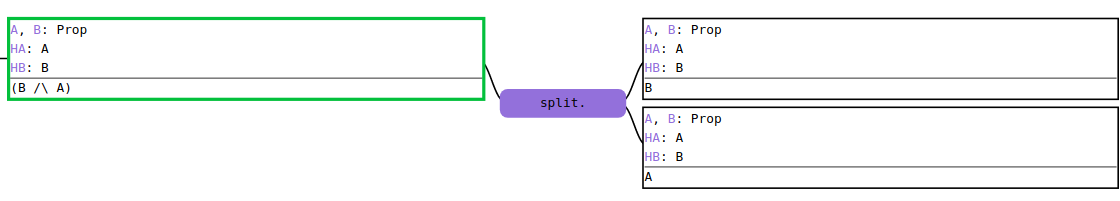
\includegraphics[width=\textwidth]{proof-tree}{\parfillskip=0pt\par}
\caption{Proof-tree view: three obligations nodes and one tactic node}%
\label{proof-tree-view-nodes}
\end{figure*}

When the user enters a proof, a single, root obligation node is created.  This
node corresponds to the current, single proof obligation.  In order to progress,
the user will invoke a tactic.  When they do, a tactic node will be inserted as
a child of the current obligation node, thus denoting that this tactic was ran
from that context.  Depending on the outcome of the tactic execution, one of the
following will happen:

\begin{itemize}

  \item if the tactic yields sub-obligations, these are added as children to the
tactic node, and the focus shifts to the first such sub-obligation,

  \item if the tactic yields no obligation (i.e.\ concludes the current
obligation), then the solved sub-trees are visually folded, and the focus moves
to the next pending obligation, if any.  When there are none, it means the proof
is completed.

\end{itemize}

If the current obligation resulted from the execution of a tactic (i.e. for all
obligations but the root one), the user may backtrack their decision and return
to the state prior to the execution of the parent tactic.
